%Controllata punteggiatura e errori di battitura 

\chapter{Esperimento}

\section{Goal dell'Esperimento}

Come evidenziato nel Capitolo~\ref{sec:capitolo4}, l’impiego dei Large Language Models (LLM) nel dominio dell’ingegneria del software si è concentrato prevalentemente sull’identificazione di \textit{code smells} e vulnerabilità locali. Sebbene studi recenti, come il prototipo MicroPAD, abbiano iniziato a dimostrare la fattibilità di utilizzare gli LLM per riconoscere pattern architetturali positivi a partire da file di configurazione (IaC), l’efficacia di tali modelli nel rilevamento di difetti complessi a livello di sistema distribuito, ovvero gli anti-pattern architetturali nelle architetture a microservizi (MSA), analizzando l’intera \textit{codebase}, rappresenta un ambito di ricerca ancora largamente inesplorato.

Alla luce di queste mancanze, l'obiettivo principale del presente esperimento è valutare empiricamente le capacità e i limiti degli LLM di ultima generazione nell'individuare specifici AP (sia architetturali sia appartenenti ad altre categorie) all'interno di \textit{codebase} reali di grandi dimensioni.

%Le lascio in inglese?
Nello specifico, l'esperimento è stato progettato per rispondere alle seguenti \textit{Research Questions (RQ)}:
\begin{itemize}
    \item \textbf{RQ1: Quanto sono efficaci gli LLM nel rilevare gli anti-pattern nelle MSA?}

    L'obiettivo è misurare l'efficacia pura dei modelli nel riconoscere difetti architetturali, fornendo in ingresso un input elaborato mediante \textit{Repomix} e valutando l'output analizzando metriche standard, come Precision, Recall e F1, rispetto a una \textit{ground truth} validata manualmente.
    
    \item \textbf{RQ2: Come si confrontano gli LLM con gli strumenti di analisi statica allo stato dell’arte per il rilevamento degli anti-pattern nelle MSA?}

    Successivamente, l'esperimento si propone di confrontare criticamente le performance ottenute dagli LLM con quelle prodotte da strumenti di detection considerati lo stato dell'arte in questo dominio. In particolare, i risultati dei modelli verranno comparati con quelli generati da MARS, al fine di comprendere se l'approccio degli LLM possa superare, eguagliare o quantomeno complementare i limiti strutturali tipici di tali strumenti.

\end{itemize}
Per raggiungere questi obiettivi, lo studio prevede l'esecuzione di test comparativi su un set eterogeneo di repository open-source, impiegando tecniche avanzate di \textit{Prompt Engineering} e strumenti di gestione dei dati di input (come \textit{Repomix}) per ridurre le problematiche associate alla dimensione del contesto e alla sua elaborazione.

\subsection{Selezione degli LLM}

Per condurre l'esperimento sono stati selezionati tre modelli nel panorama attuale: \textbf{Qwen 3.5 Plus} \cite{alibaba2026qwen35}, \textbf{Gemini 3.0 Pro} \cite{deepmind2026gemini31} e \textbf{ChatGPT 5.2} \cite{openai2025gpt52}. La scelta di questi specifici modelli è stata guidata principalmente da un requisito tecnico fondamentale, necessario per affrontare le complessità dell'analisi architetturale: la \textbf{gestione di finestre di contesto estese (\textit{Large Context Windows})}.

Come analizzato nel Capitolo~\ref{sec:capitolo4}, l'analisi di un'architettura a microservizi richiede l'ingestione di interi repository. I modelli selezionati dispongono di capacità di elaborazione molto elevate, che consentono di processare l'intera \textit{codebase} senza ricorrere a complessi e potenzialmente rischiosi meccanismi di frammentazione del codice. Nello specifico, come riassunto nella Tabella~\ref{tab:llm-selection}, Gemini e Qwen offrono una finestra di contesto pari a 1.000.000 di token, mentre ChatGPT 5.2 supporta contesti fino a 400.000 token. Durante i test empirici, tali dimensioni si sono mostrate generalmente adeguate all'elaborazione di progetti di grandi dimensioni, senza errori espliciti o interruzioni del servizio.

Va inoltre osservato che, nel caso di ChatGPT, ai limiti della finestra di contesto del modello si affiancano vincoli propri della piattaforma di caricamento dei documenti: i file di testo e i documenti caricati in una conversazione o in un GPT sono soggetti a un limite di 2 milioni di token per file, oltre al limite dimensionale di 512 MB \cite{openai_file_uploads_faq}. Tale soglia costituisce quindi un vincolo pratico all'ingestione di repository o documentazione particolarmente estesi, distinto dalla finestra di contesto effettivamente disponibile al modello \cite{openai_file_uploads_faq}.

Durante i test empirici, si è tuttavia osservata un'eccezione metodologicamente rilevante: per tre repository analizzati, lo strumento di aggregazione del codice (Repomix \cite{repomix2026}) ha stimato un peso in token nominalmente superiore alla soglia dei 400.000 token attribuita a ChatGPT 5.2. Nonostante ciò, il modello ha processato l'input senza restituire errori espliciti di superamento del limite di contesto. Tale risultato va interpretato con attenzione. In primo luogo, la stima fornita da Repomix ha carattere approssimativo e può non coincidere con il conteggio effettivo dei token operato dal sistema. In secondo luogo, l'assenza di errori visibili non consente di escludere che il modello abbia adottato strategie interne non osservabili per la gestione dell'input, con possibili effetti sulla completezza dell'elaborazione. Di conseguenza, pur in assenza di fallimenti espliciti, non può essere esclusa una perdita informativa.

La Tabella~\ref{tab:llm-selection} riassume le specifiche tecniche principali dei tre modelli scelti.

\begin{table}[H]
    \centering
    \caption{Lista LLM utilizzati.}
    \label{tab:llm-selection}
    \vspace{0.2cm}
    \renewcommand{\arraystretch}{1.3}
    \resizebox{\textwidth}{!}{%
    \begin{tabular}{l l c}
        \toprule
        \textbf{Modello} & \textbf{Sviluppatore} & \textbf{Context Window (Token)} \\
        \midrule
        \textbf{Gemini 3.0 Pro} & Google DeepMind & 1.000.000 \\
        \textbf{Qwen Plus 3.5}  & Alibaba Cloud   & 1.000.000 \\
        \textbf{ChatGPT 5.2}    & OpenAI          & 400.000 \\
        \bottomrule
    \end{tabular}%
    }
\end{table}

\subsection{Repository analizzate}

Per valutare l'efficacia degli LLM nell'identificazione degli anti-pattern, è stato selezionato un dataset composto da 13 repository \textit{open-source} basate su architettura a microservizi. Tale dataset, le cui metriche dimensionali sono riassunte nella Tabella~\ref{tab:repositories}, è caratterizzato da un'elevata eterogeneità: comprende infatti sia progetti dimostrativi di piccole dimensioni (poche centinaia di linee di codice), sia sistemi complessi assimilabili a contesti \textit{enterprise} (con decine di microservizi e quasi 90.000 linee di codice, come nel caso di \textit{Micro Company} e \textit{Lakeside Mutual}).

\begin{table}[H]
    \centering
    \caption{Elenco delle repository a microservizi analizzate nell'esperimento, con le relative metriche dimensionali.}
    \label{tab:repositories}
    \vspace{0.2cm}
    \renewcommand{\arraystretch}{1.2}
    \resizebox{\textwidth}{!}{%
    \begin{tabular}{l c c c c}
        \toprule
        \textbf{Repository} & \textbf{Microservices} & \textbf{Files} & \textbf{LOC} & \textbf{Reference} \\
        \midrule
        Apollo & 9 & 68 & 29.510 & \cite{ApolloRepository} \\
        TeaStore & 3 & 62 & 5.073 & \cite{TeaStoreRepository} \\
        Spring Cloud Microservice Movie & 4 & 33 & 885 & \cite{SpringCloudMicroserviceMovieRepository} \\
        Freddy's BBQ & 6 & 35 & 1.752 & \cite{FreddysBBQRepository} \\
        Piggymetrics & 4 & 88 & 3.176 & \cite{PiggymetricsRepository} \\
        FTGO & 9 & 257 & 8.239 & \cite{FTGORepository} \\
        Spring Boot Microservices & 2 & 4 & 116 & \cite{SpringBootMicroservicesRepository} \\
        Lakeside Mutual & 9 & 424 & 89.477 & \cite{LakesideMutualRepository} \\
        Warehouse Microservice & 6 & 222 & 4.623 & \cite{WarehouseMicroserviceRepository} \\
        Qbike & 5 & 77 & 2.057 & \cite{QbikeRepository} \\
        Microservice Demo & 3 & 38 & 1.766 & \cite{MicroserviceDemoRepository} \\
        CQRS Microservice Sampler & 3 & 26 & 1.028 & \cite{CQRSMicroserviceSamplerRepository} \\
        Micro Company & 17 & 244 & 90.315 & \cite{MicroCompanyRepository} \\
        \bottomrule
    \end{tabular}%
    }
\end{table}

\subsection{Ground truth manuale}
A tale scopo, per le tredici repository selezionate è stata utilizzata la ground truth (GT) manuale resa disponibile dallo studio MARS \cite{MARS}. È importante precisare che tale ground truth non è stata generata automaticamente dal tool MARS, bensì costruita manualmente dagli autori dello studio attraverso un processo di validazione umana. 
MARS utilizza il GT come strumento di validazione del proprio output.
I dati completi relativi alla \textit{Ground Truth} sono pubblicamente accessibili e consultabili al riferimento \cite{GT_mars}.

\section{Procedura sperimentale}

Come illustrato nel diagramma in Figura~\ref{fig:pipeline}, l'architettura dell'esperimento è stata formalizzata in un processo sistematico e riproducibile. L'esecuzione si articola in quattro fasi, che rispecchiano l'esatta evoluzione cronologica dello studio: dall'analisi degli LLM fino al successivo confronto con MARS.

\vspace{0.8em}
\begin{figure}[ht]
    \centering
    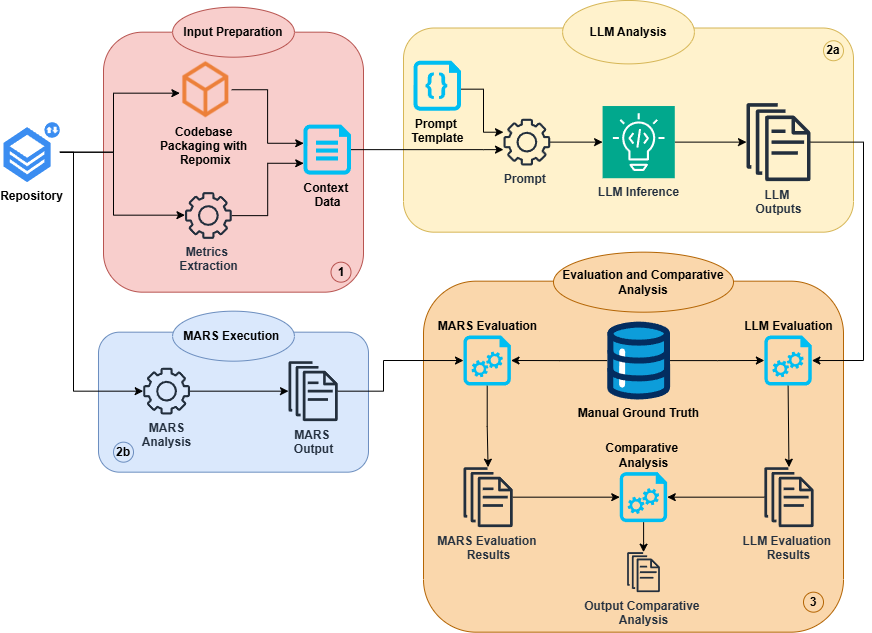
\includegraphics[width=1.0\textwidth]{img/pipeline_d2.png}
    \caption{Pipeline dell'esperimento.}
    \label{fig:pipeline}
\end{figure}

Di seguito si riportano le varie fasi della pipeline dell'esperimento:
\begin{description}
    \item[Fase 1: Input Preparation]
    \hfill \\
    In questa fase, è fornito in input a \textit{Repomix} e allo script di estrazione delle metriche quantitative la repository selezionata. 
    Mediante \textit{Repomix} incapusuliamo la repository con una struttura LLM-friendly, generando un unico artefatto testuale ottimizzato. 
    Parallelamente è eseguita la sotto-fase di \textit{Metrics Extraction} mediante la quale con uno script Python, si vanno ad estrarre i parametri quantitativi (es. LOC, numero di file e di servizi). 
    I due output delle due sotto-fasi generano i \textit{Context Data}, ovvero la base di conoscenza sulla quale il modello dovrà ragionare per rilevare gli anti-pattern. 
    
    \item[Fase 2a: LLM Analysis]
    \hfill \\
    I \textit{Context Data} sono combinati al \textit{Prompt Template} per generare il \textit{Prompt} finale che verrà sottoposto ai modelli. 
    Il \textit{Prompt Template} ha in generare una struttura fissa; per ciascun anti-pattern cambiano esclusivamente la definizione, l'esempio e quando necessario, alcune \textbf{regole aggiuntive} specifiche dell'AP analizzato.
    Realizzato il \textit{Prompt}, si procede alla sotto-fase di \textit{LLM Inference}, nella quale i tre modelli selezionati (ChatGPT, Gemini e Qwen) elaborano l'input fornito generando gli \textit{LLM Outputs} della detection.

    
    \item[Fase 2b: MARS Execution]
    \hfill \\
    Parallelamente al processo visto nelle prime due fasi, viene eseguito il tool di analisi statica MARS, generando la baseline necessaria per il confronto con gli output dei modelli.

    \hfill \\
    \item[Fase 3: Evaluation and Comparative Analysis]
    \hfill \\
    Gli output degli LLM sono successivamente analizzati nella sotto-fase di \textit{LLM Evaluation}, nella quale si confrontano i risultati ottenuti con una \textit{Manual Ground Truth} per ottenere di fatto delle metriche qualitative (\textit{Precision} \textit{Recall} \textit{F1-score}) mediante le quali possiamo comprendere a pieno quanto i modelli sono precisi e di conseguenza rispondere alla \textbf{prima RQ}.
    Analogamente a quanto fatto con gli LLM, nella sotto-fase di \textit{MARS Evaluation} vengono valutati i risultati di ottenuti da MARS. 
    Ottenute le metriche qualitative riferite agli output degli LLM e di MARS, si può procedere al confronto diretto tra i due approcci, ottenendo di conseguenza risposta alla \textbf{seconda RQ}.
\end{description}

Nel seguito vengono approfondite alcune sotto-fasi del processo, al fine di chiarire in modo puntuale le modalità con cui sono stati ottenuti i risultati che saranno oggetto di discussione più avanti.

\subsection{Incapsulamento repository con Repomix (Fase 1)}

In una fase preliminare dell'esperimento, si è cercato di fornire agli LLM una rappresentazione astratta dell'architettura. Per farlo, sono stati testati strumenti open-source di analisi statica come \textit{code2dfd} e \textit{rad-source}, con l'obiettivo di estrarre diagrammi di flusso dei dati (DFD) e grafi delle dipendenze \cite{Static_Tool, cloudhubs_rad_source, Code2DFD23}. Tuttavia, questa strategia ha mostrato due limiti principali.

In primo luogo, ciascuno strumento catturava soltanto uno specifico sottoinsieme di informazioni, restituendo quindi una rappresentazione inevitabilmente parziale del sistema. Tale limite non consentiva di includere tutti gli elementi necessari per individuare anti-pattern legati a configurazioni o logiche di comunicazione inter-servizio. In secondo luogo, per avere una visione completa che fosse idonea per ogni AP, sarebbe stato necessario usare più strumenti contemporaneamente, introducendo un ulteriore livello di complessità per normalizzare e unire output molto diversi in un unico file per l'LLM.

Per evitare questa frammentazione, si è deciso di sfruttare l'ampia finestra di contesto dei modelli moderni per fornire in input l'intera \textit{codebase}. È stato quindi adottato \textbf{Repomix}, uno strumento open-source progettato per aggregare l'intero contenuto di una repository software in un singolo file di testo, strutturato appositamente per essere compreso dai \textit{Large Language Models} \cite{repomix2026}.

L'uso di Repomix è stato guidato da un file di configurazione personalizzato (\texttt{repomix.config.json}) per ottimizzare il testo ed escludere il codice non rilevante per l'analisi architetturale \cite{repomix2026}. Nello specifico, sono state applicate queste regole \cite{repomix2026}:

\begin{itemize}
    \item \textbf{Pulizia del codice:} sono stati rimossi i commenti e le righe vuote (\texttt{removeComments: true}, \texttt{removeEmptyLines: true}) per massimizzare la densità delle informazioni. Questa scelta è stata motivata anche dalla necessità di garantire un confronto equo. I commenti, infatti, possono contenere suggerimenti preziosi sulle scelte architetturali che agevolerebbero il modello; tuttavia, non essendo presenti in egual misura in tutti i progetti, lasciarli intatti avrebbe introdotto un \textit{bias} valutativo, alterando le prestazioni di \textit{detection} (migliori o peggiori) in base al livello di documentazione interna della singola \textit{codebase}.
    
    \item \textbf{Numerazione delle righe:} è stata attivata l'opzione per mostrare i numeri di riga (\texttt{showLineNumbers: true}), fondamentale per permettere all'LLM di indicare con precisione in quale file e a quale riga si trova un potenziale anti-pattern. Inoltre, tale funzione si è rivelata utile per controllare in maniera manuale alcuni risultati, potendo rintracciare facilmente gli artefatti all'interno della codebase.
    
    \item \textbf{Esclusioni mirate:} invece di usare le regole base del sistema di controllo di versione (\texttt{useGitignore: false}), è stata definita una lista personalizzata dei file da ignorare mediante l'opzione  (\texttt{customPatterns}). Oltre a file binari, librerie esterne (es. \texttt{node\_modules}) e documentazione, sono state escluse interamente le suite di \textbf{testing} (directory \texttt{tests/}, file \texttt{*Test.java}, ecc.). I file di test non contengono la logica strutturale dei microservizi; pertanto, la loro esclusione ha permesso di risparmiare una grande quantità di spazio, facilitando il lavoro di elaborazione dei modelli.
    Il file di configurazione utilizzato per Repomix è reperibile al seguente riferimento \cite{barbato_tesi_llm_scripts}.
    
    
\end{itemize}

Il file finale è stato generato in formato testo semplice (\texttt{style: "plain"}) mantenendo intatta la struttura delle directory (\texttt{directoryStructure: true}), per aiutare il modello a orientarsi tra i vari moduli e capire come sono separati i microservizi.

Infine, per quanto riguarda il consumo di spazio, Repomix include una funzione di stima dei \textit{token}. Nel file di configurazione è stato impostato l'algoritmo di codifica \texttt{o200k\_base} (lo standard utilizzato dai modelli OpenAI più recenti). È importante precisare che i tre modelli scelti per l'esperimento (ChatGPT, Gemini e Qwen) utilizzano \textit{tokenizer} proprietari differenti e quindi calcolano i \textit{token} in modo leggermente diverso l'uno dall'altro. Tuttavia, l'uso dello standard OpenAI è servito unicamente come metrica di stima di riferimento: ha permesso di verificare rapidamente che la dimensione totale del file generato per ogni repository fosse ampiamente contenuta all'interno della grande finestra di contesto (fino a 1 milione di \textit{token}) supportata da tutti i modelli in fase di inferenza.
Nei rari casi in cui la dimensione della repository eccedeva i limiti del modello, non sono stati osservati cali percepibili nelle prestazioni di detection. Questo risultato suggerisce che, nel setup sperimentale adottato, il sistema abbia gestito input di grandi dimensioni senza manifestare errori espliciti, pur senza consentire conclusioni definitive sui meccanismi interni di elaborazione. Tuttavia, tale interpretazione è basata esclusivamente su evidenze empiriche e non su dettagli implementativi esplicitamente documentati.

\subsection{Estrazione metriche (Fase 1)}

L'output testuale generato da Repomix offre una visione completa della \textit{codebase}, ma lo strumento non fornisce la possibilità di effettuare il calcolo e l'aggregazione di metriche strutturali relative alla repository, come il numero esatto di righe di codice, classi o metodi raggruppati per singolo microservizio. D'altra parte, richiedere a un LLM di ricavare tali informazioni direttamente dal file generato da repomix risulta essere complesso e aumenterebbe inutilmente il carico in termini computazionali del modello.

Poiché l'identificazione di anti-pattern dimensionali, come il \textit{MegaService} o il \textit{NanoService}, richiede soglie numeriche precise, si è scelto di alleggerire il compito del modello fornendogli dati già pre-calcolati. Di conseguenza, parallelamente all'esecuzione di Repomix, è stato sviluppato uno script Python custom incaricato di eseguire un'analisi statica leggera; il codice sorgente completo dello strumento è disponibile nel repository GitHub del progetto \cite{barbato_tesi_llm_scripts}. L'obiettivo dello \textit{script} è estrarre metriche software oggettive per ciascun microservizio e restituirle in un formato strutturato (\texttt{JSON}).

Il funzionamento dello \textit{script} si articola in due macro-operazioni principali:

\vspace{0.5em}
\noindent\textbf{1. Rilevamento dinamico dei microservizi (\textit{Service Discovery})}\\
Lo \textit{script} analizza la struttura della \textit{codebase} alla ricerca di file di configurazione tipici dei vari ecosistemi di sviluppo (ad esempio \texttt{pom.xml} per Maven, \texttt{build.gradle} per Gradle, \texttt{package.json} per frontend/Node.js e \texttt{go.mod} per Go). Questa logica consente di identificare automaticamente i confini di ciascun servizio, escludendo i file di aggregazione generale, come i POM aggregatori.
Di seguito si riporta un estratto della logica di rilevamento:

\vspace{0.5em}
\noindent\textit{Codice 1: Frammento per il rilevamento dinamico dei microservizi.}
\begin{Verbatim}[breaklines=true, breakanywhere=true]
def find_microservices(project_root: Path):
    services = {}
    # Rilevamento Maven (escludendo i pom aggregatori)
    for pom in project_root.rglob("pom.xml"):
        if not is_excluded_path(pom) and not is_aggregator_pom(pom):
            add_service(pom.parent, "maven")
            
    # Rilevamento Node/Frontend (evitando i node_modules)
    for pkg in project_root.rglob("package.json"):
        if not is_excluded_path(pkg) and "node_modules" not in pkg.parts:
            add_service(pkg.parent, "node")
            
    # Rilevamento Go, Python, Docker...
    return services
\end{Verbatim}
\vspace{0.5em}

\noindent\textbf{2. Conteggio robusto delle metriche (LOC, Classi, Metodi)}\\
Una volta delimitati i servizi, lo \textit{script} calcola le metriche dimensionali. Per garantire l'accuratezza delle \textit{Lines of Code} (LOC), è stato implementato un \textit{parser} in grado di ignorare le righe vuote e i commenti (sia in linea sia a blocco), supportando sintassi eterogenee (stile C, HTML e Hash). Lo strumento utilizza inoltre espressioni regolari per contare il numero di classi, metodi e costruttori definiti nel codice, discriminando tra i vari linguaggi di programmazione supportati (Java, Kotlin, Python, Go, TypeScript/JavaScript). È stata inoltre integrata una logica per evitare il doppio conteggio nei casi di microservizi annidati (\textit{cross-service exclusion}).


\vspace{0.5em}
L'output finale di questo processo è un file \texttt{.json}  che racchiude tutte le informazioni necessarie per ogni microservizio individuato (come i totali di LOC, classi e metodi). È importante osservare che il file in questione non viene fornito al modello per ogni AP. Al fine di ottimizzare l'analisi, si è preferito fornire al modello lo stretto necessario e di conseguenza tale file viene aggiunto ai \textbf{Context Data (3a)} solo per gli AP dimensionali (\textit{NanoService} e \textit{MegaService}).

Per la rilevazione di tutti gli altri AP, il modello si basa unicamente sul codice sorgente compattato, evitando di sovraccaricare il \textit{prompt} con metriche numeriche non pertinenti al \textit{task} specifico.

\subsection{Costruzione del Prompt e Input al Modello (Fase 2a)}
\vspace{1em}
Per garantire la totale riproducibilità dell'esperimento e standardizzare le risposte, è stato ingegnerizzato un \textit{Template} base da cui sono stati derivati i singoli \textit{prompt}. Come si evince dal seguente schema strutturale, le istruzioni, i vincoli di rilevamento e i formati di \textit{output} sono stati mantenuti rigorosamente identici per tutte le esecuzioni, variando esclusivamente la definizione teorica del difetto ricercato.

\vspace{1em}
\noindent\textit{Codice 3: Struttura base del Prompt Template utilizzato per le inferenze.}
\vspace{0.5em}

\begin{mdframed}[linewidth=0.8pt, innermargin=10pt, outermargin=0pt]
\sffamily \small \raggedright
Act as an expert microservice architecture analyst and reverse-engineering researcher tasked with detecting a specific Architectural Anti-Pattern in a provided software repository or codebase.\\

You will receive one or more input files describing a software system. Treat these inputs as the sole source of truth; do not assume the presence of any missing files or behaviors. Never respond with UNKNOWN.\\

Your task is to analyze the entire provided artifacts and determine whether the specified microservice architectural anti-pattern is \textbf{PRESENT} or \textbf{ABSENT}, strictly according to the exact definition and example given below.\\

\vspace{0.5em}
\textbf{ANTI-PATTERN}\\
\textbf{Name:} [NOME ANTI-PATTERN]\\
\textbf{Definition:} [DEFINIZIONE FORMALE DELL'AP]\\
\textbf{Example:} [ESEMPIO DESCRITTIVO OPPURE BASATO SU INPUT/OUTPUT]\\

\vspace{0.5em}
\textbf{Detection Constraints:}\\
- Follow only the provided definition and example without generalization or extension.\\
- Translate the definition into observable indicators only if explicitly implied.\\
- Cross-reference all provided inputs including services, modules, endpoints, dependencies, shared resources, and deployment descriptors.\\
- If any required information is missing, ambiguous, or unverifiable from the artifacts, output \textbf{ABSENT} and specify exactly what is missing.\\
- The anti-pattern name in your output must exactly match the provided Name.\\

\vspace{0.5em}
\textbf{Reasoning Instructions:}\\
- Think carefully and exhaustively, based solely on the provided definition and example.\\
- Do not reveal your internal reasoning steps or intermediate thoughts.\\

\vspace{0.5em}
\textbf{Output Format (ONLY these sections, in this order, with no additional content):}\\

\textbf{ANTI-PATTERN:} [Exact Name]\\
\textbf{STATUS:} PRESENT | ABSENT\\

\vspace{0.5em}
\textbf{SUMMARY (1-2 lines):}\\
- \textbf{PRESENT:} Briefly describe what the anti-pattern is and where it manifests.\\
- \textbf{ABSENT:} Briefly explain why the analyzed artifacts do not meet the definition or example.\\

\vspace{0.5em}
\textbf{RATIONALE (max 4 bullets):}\\
- \textbf{PRESENT:} Reasons why observed features match the definition/example; key indicators.\\
- \textbf{ABSENT:} Which required conditions are not met or unverifiable from the artifacts.\\

\vspace{0.5em}
\textbf{SUPPORTING INDICATORS (only if PRESENT):}\\
- Provide 1 to 4 concrete observations anchored to specific artifacts (including filename and line number if available).\\
- Additional relevant observations as necessary.\\

\vspace{0.5em}
\textbf{SERVICES / COMPONENTS INVOLVED:}\\
- \textbf{PRESENT:} Explicitly list affected services or components identifiable from the artifacts.\\
- \textbf{ABSENT:} None identified.\\

\vspace{0.5em}
Ensure clarity, precision, and strict adherence to the instructions throughout.
\end{mdframed}
\vspace{1em}

\vspace{1em}

Per la costruzione dei \textit{prompt}, si è scelto di combinare diverse tecniche con l'obiettivo di guidare i modelli in modo preciso, evitando di condizionarne le scelte o di introdurre involontariamente dei \textit{bias} durante l'analisi:

\begin{itemize}
    \item \textbf{Role Prompting:} Chiedere all'LLM di agire come un esperto (\textit{"Act as an expert microservice architecture analyst..."}) lo aiuta a calarsi nel giusto contesto, spingendolo ad adottare il rigore tipico di un ingegnere del software.
    
    \item \textbf{Zero-shot ancorato a definizione ed esempio:} il prompt utilizzato prevede che il modello si basi e faccia fede solo alle informazioni derivate dalla \textit{definizione} e dall'\textit{Example} per la detection. Sono stati usati \textit{Example} descrittivi e narrativi (come lo scenario di un \textit{e-commerce}) con l'aggiunta, in alcuni casi, di alcuni frammenti di codice per aiutare il modello nell'identificazione sintattica di alcuni AP. 
    Si specifica che per alcuni \textit{prompt} la presenza della sezione \textit{Example} non portava a reali vantaggi; di conseguenza, per alleggerire il testo, in questi casi è stata omessa.
    
    \item \textbf{Constraint-Based Prompting:} Serve a "ingabbiare" il comportamento del modello per evitare risposte imprevedibili o formattazioni sballate. Abbiamo usato vincoli strutturali rigidi (come \textit{"Never respond with UNKNOWN"} e una precisa struttura per l'\textit{output}).
    
    \item \textbf{Rule-Based Prompting:} È stato utilizzato in modo molto mirato senza eccedere per gestire specifiche eccezioni di dominio. L'obiettivo non era pilotare il modello passo dopo passo, ma fornirgli solo i confini essenziali su cosa escludere a priori (ad esempio, i file di test o i componenti infrastrutturali). Questo ha permesso di evitare i falsi positivi più banali, lasciando comunque all'LLM la massima libertà e autonomia nell'individuare i difetti veri e propri.
    
    \item \textbf{Chain-of-Thought (CoT):} Abbiamo chiesto al modello di ragionare a fondo prima di decidere, ma di tenere per sé i passaggi intermedi (\textit{"Do not reveal your internal reasoning steps"}). In questo modo otteniamo un'analisi profonda senza "sporcare" il testo finale generato.
    
\end{itemize}

La totalità dei prompt utilizzati è consultabile al riferimento \cite{barbato_tesi_llm_scripts}.

\vspace{1em}
\subsubsection*{Selezione delle definizioni e regole}
Un passaggio importante ha riguardato la scelta delle definizioni degli anti-pattern. Le definizioni formali proposte nel \textit{paper} originale di Cerny et al. risultavano a volte troppo stringenti o complesse per essere recepite correttamente da un LLM, con conseguente abbassamento della recall. Per agevolare il compito del modello, in alcuni casi abbiamo preferito utilizzare le definizioni fornite dal \textit{paper} di MARS, che si sono rivelate più pratiche e dirette. La \textbf{Tabella~\ref{tab:ap_definitions}} riassume le definizioni esatte usate per ogni anti-pattern e la loro provenienza bibliografica.

\begin{table}[H]
    \centering
    \scriptsize
    \renewcommand{\arraystretch}{1.3}
    \caption{Definizioni degli Anti-Pattern utilizzate nei Prompt.}
    \label{tab:ap_definitions}
    \begin{tabular}{| p{3cm} | p{8.5cm} | p{3cm} |}
        \hline
        \textbf{Anti-Pattern} & \textbf{Definizione fornita al Modello} & \textbf{Fonte} \\ \hline
        
        \textbf{Wrong Cuts} & The system is decomposed into microservices following technical aspects, such as the presentation layer, business layer, and data access layer. Microservice should encapsulate functionalities fulfilling a single purpose. & Cerny et al. \cite{CernyCatalogo} \\ \hline

        \textbf{Nano-Service} & The service is too fine-grained and only has a few operations. Its overhead (communications, maintenance, and so on) outweighs its utility. Nanoservices cause fragmented logic and performance issues. & Cerny et al. \cite{CernyCatalogo} \\ \hline

        \textbf{Shared Libraries} & Microservices should not share runtime libraries or source code that contain business logic or domain-specific functionality. Sharing such internal libraries breaks service boundaries and reduces independence. & Cerny et al. \cite{CernyCatalogo} \\ \hline

        \textbf{Hardcoded \newline Endpoint} & Microservice IP addresses, ports, or full endpoint URLs are explicitly specified in source code, configuration files, or environment variables in a way that couples clients to a specific address/port. & Cerny et al. \cite{CernyCatalogo} \\ \hline

        \textbf{Manual \newline Configuration} & Configuration of instances, services, and hosts is done manually. Microservices should separate the core codebase from the configuration management to enable automation. & Cerny et al. \cite{CernyCatalogo} \\ \hline

        \textbf{No API Gateway} & When a microservice-based system lacks an API gateway, the clients of the application necessarily have to invoke its microservices directly. The system lacks a unified entry point for centralized routing. & Cerny et al. \cite{CernyCatalogo} \\ \hline

        \textbf{Mega-Service} & Microservices should be small, independent, independently deployable units and serve a single purpose. A mega service has a high number of lines of code, modules, or files, as well as a high fan-in. & Cerny et al. \cite{CernyCatalogo} \\ \hline

        \textbf{Shared \newline Persistency} & Different microservices are accessing the same database/schema (often the same tables/entities). In the worst kind, different services use the same entities of a service. & Cerny et al. \cite{CernyCatalogo} \\ \hline

        \textbf{No API \newline Versioning} & In a microservice architecture, if one or more services expose REST APIs to clients without any form of versioning (path-based, header-based, or query parameter), then the system suffers from this. & Cerny et al. \cite{CernyCatalogo} \\ \hline

        \textbf{No Health Check \newline (NHC)} & This antipattern describes microservices that are not periodically health-checked. Unavailable microservices may not be noticed, leading to timeouts and other errors. & MARS \cite{MARS} \\ \hline

        \textbf{Insufficient \newline Monitoring} & Performance and failure of the microservices are not tracked. Failures become more difficult to catch and tracking performance issues become more tedious. A solution is to adopt a global monitoring tool. & Cerny et al. \cite{CernyCatalogo} \\ \hline

        \textbf{Timeouts \newline (TO)} & This antipattern happens when timeout values are set and hard-coded in HTTP requests, which leads to unnecessary disconnections or delays. & MARS \cite{MARS} \\ \hline

        \textbf{Multiple Service \newline Instances Per Host} & A single host contains multiple microservices instances deployed to the same host. Microservices have to share the same resources that are available inside the host. & Cerny et al. \cite{CernyCatalogo} \\ \hline

        \textbf{Local Logging \newline (LL)} & This antipattern results from microservices having their own logging mechanism, which prevents aggregation and analyses of their logs and the monitoring and recovery of systems. & MARS \cite{MARS} \\ \hline

        \textbf{No CI/CD} & Continuous integration and delivery are important for microservices to automate repetitive steps during testing and deployment. Not using CI/CD undermines the microservice architectural style. & MARS \cite{MARS} \\ \hline

        \textbf{Cyclic \newline Dependency} & A cyclic chain of calls between services exists. When
        two or more services depend on each other directly or
        indirectly. The services involved in a dependency cycle
        can be hard to release and maintain. This dependency
        implies that there are two pieces of code that are
        highly coupled to each other in a direct or indirect way.
        This situation might suggest that the responsibilities are
        not separated correctly across services. Various cyclic
        dependency shapes can be recognized. This leads to
        problems with deployment, scalability, and co-change
        coupling. & Cerny et al. \cite{CernyCatalogo} \\ \hline
        
    \end{tabular}
\end{table}
\vspace{1em}

Inoltre, pur mantenendo lo stesso \textit{template} di base, per alcuni AP è stato necessario aggiungere degli esempi specifici per guidare il modello e limitare i falsi positivi:

\begin{itemize}
    \item \textbf{Hardcoded Endpoint:} Abbiamo strutturato maggiormente il prompt \textit{zero-shot}, arricchendo la definizione dell'anti-pattern con esempi descrittivi e operativi più dettagliati. Tali esempi non rappresentano casi di classificazione già risolti, ma servono a delimitare con maggiore precisione il perimetro dell'anti-pattern, chiarendo quali endpoint debbano essere considerati validi ai fini della detection e quali invece debbano essere esclusi. Sono state inoltre introdotte delle regole di esclusione, ad esempio per endpoint presenti solo in file di test, documentazione API, placeholder privi di valore concreto, endpoint infrastrutturali o riferimenti a service discovery, con l'obiettivo di ridurre il numero di falsi positivi.
    
    \item \textbf{Nano-Service e Mega-Service:} Per valutare la dimensione dei microservizi, abbiamo esplicitamente escluso dall'analisi i servizi infrastrutturali (come \textit{Eureka} o \textit{Zipkin}) e le app di \textit{demo} (i classici \textit{hello-world}). Il motivo è puramente architetturale: i servizi infrastrutturali hanno spesso pochissimo codice scritto a mano, semplicemente perché delegano tutto il lavoro al \textit{framework}. Segnalarli come "Nano-Service" sarebbe un errore concettuale, poiché questi anti-pattern servono a valutare se la logica di \textit{business} è stata frammentata male, non a giudicare l'impalcatura tecnica di base.

    \item \textbf{Shared Libraries:} Anche per questo anti-pattern è stato necessario arricchire il \textit{prompt} con precisazioni operative e semantiche, pur mantenendo un'impostazione \textit{zero-shot}. Al modello non sono infatti stati forniti esempi completi di classificazione già risolti, ma indicazioni volte a delimitare meglio il significato dell'anti-pattern e i relativi casi di confine.

    Una definizione troppo generica, nelle fasi preliminari dell'esperimento, portava il modello a classificare erroneamente come AP anche librerie condivise di natura tecnica. Per tale motivo, è stato esplicitato che la semplice presenza di moduli o cartelle denominati \texttt{common}, \texttt{shared}, \texttt{core} o \texttt{domain}, anche se importati da più servizi, non costituisce di per sé evidenza sufficiente dell'anti-pattern. Tali moduli devono essere considerati rilevanti solo quando contengono effettiva logica di \textit{business} o funzionalità \textit{domain-specific}.

    
\end{itemize}

\subsection{Esecuzione e Inferenza degli LLM (Fase 2a)}

Una volta completata l'aggregazione del \textit{Context Data} e del \textit{Prompt Template}, il documento testuale unificato è stato sottoposto alla fase di inferenza. Per l'esperimento sono stati impiegati tre modelli linguistici di ultima generazione: ChatGPT, Gemini e Qwen.

Complessivamente, la procedura sperimentale ha comportato 624 esecuzioni indipendenti dei modelli linguistici, derivanti dalla combinazione dei 16 anti-pattern analizzati, delle 13 repository del dataset e dei 3 LLM selezionati. Questo volume di inferenze contribuisce a dare robustezza al confronto sperimentale e rende esplicita la scala effettiva della valutazione svolta.

La progettazione di questa fase ha richiesto un'attenzione metodologica particolare per garantire rigore sperimentale e indipendenza tra le singole rilevazioni. L'interazione con i modelli è avvenuta in un ambiente di esecuzione strettamente isolato (\textit{stateless}). Ogni singola valutazione è stata condotta avviando una chat temporanea dedicata, completamente priva di memoria pregressa o cronologia.

Questo approccio ha reso necessario il ricaricamento completo e da zero dell'intero \textit{prompt} (comprendente l'intera \textit{codebase} e le regole dell'anti-pattern) per ogni singola combinazione di repository, modello e anti-pattern ricercato. Sebbene questa pratica abbia richiesto il caricamento ripetuto di moli ingenti di dati e un maggior tempo materiale di esecuzione, si è rivelata una scelta metodologica obbligata per evitare che la risposta a una specifica richiesta potesse essere influenzata dalle informazioni generate o fornite in precedenza.

I \textit{Large Language Models}, infatti, tendono a sfruttare l'intero contesto conversazionale per generare le risposte. Se l'analisi di due repository distinte (o la ricerca di due anti-pattern differenti sulla stessa repository) fosse avvenuta all'interno della medesima sessione di chat, il modello avrebbe potuto manifestare dei \textit{bias} di ancoraggio. Ad esempio, avrebbe potuto erroneamente assumere la presenza di un difetto architetturale in un progetto solo perché lo aveva appena rilevato in quello precedente, oppure avrebbe potuto mescolare le regole di definizione di due anti-pattern diversi.

L'azzeramento della memoria prima di ogni esecuzione ha garantito che ogni inferenza fosse trattata come un test indipendente, basato unicamente sui dati reali della codebase analizzata in quel momento. Questo ha permesso un confronto equo tra le diverse esecuzioni e ha reso i risultati metodologicamente confrontabili anche rispetto a quelli ottenuti dallo strumento di analisi statica MARS.

È importante sottolineare che tale riproducibilità va intesa in senso controllato, poiché si riferisce alla stabilità dei risultati all'interno del setup sperimentale definito, e non alla riproducibilità assoluta del modello nel suo complesso.


